\section{Fiabilité de la sensibilité au contexte}

\begin{frame}{Rendre explicite le modèle implicite}
  \begin{minipage}{0.3\linewidth}
      \begin{figure}
        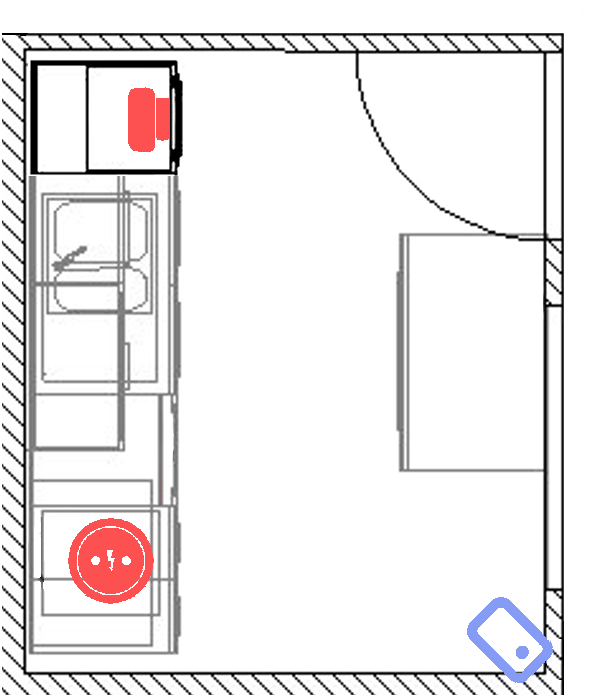
\includegraphics[scale=0.15]{use_case1.png}
      \end{figure}
    \end{minipage}
  \hfill
  \begin{minipage}{0.65\linewidth}
    %\vspace*{-25.9mm}
    \begin{coloredbox}[black]{Dépendance de présence}
      \footnotesize
      Chaque interaction (sauf présence) doit être recouverte par une interaction de présence.
      \small
      \begin{displaymath}
        \begin{array}{c}
        ~\\
        ~
        \end{array}
      \end{displaymath}
    \end{coloredbox}
    \begin{coloredbox}[black]{Non ubiquité}
      \footnotesize
      Une présence ne peut pas être simultanément détectée dans deux endroits différents.
      \small
      \begin{displaymath}
        \begin{array}{c}
         ~\\ 
         ~
        \end{array}
      \end{displaymath}
    \end{coloredbox}
  \end{minipage}
\end{frame}

\begin{frame}{Rendre explicite le modèle implicite}
  \addtocounter{framenumber}{-1}
  \begin{minipage}{0.3\linewidth}
      \begin{figure}
        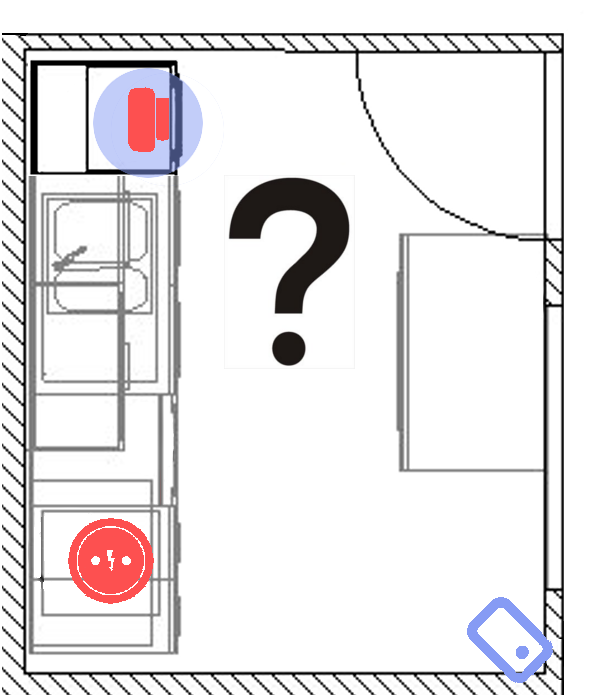
\includegraphics[scale=0.15]{use_case_issue_1.png}
      \end{figure}
    \end{minipage}
  \hfill
  \begin{minipage}{0.65\linewidth}
    %\vspace*{-25.9mm}
    \begin{coloredbox}[black]{Dépendance de présence}
      \footnotesize
      Chaque interaction (sauf présence) doit être recouverte par une interaction de présence.
      \small
      \begin{displaymath}
        \begin{array}{c}
        ~\\
        ~
        \end{array}
      \end{displaymath}
    \end{coloredbox}
    \begin{coloredbox}[black]{Non ubiquité}
      \footnotesize
      Une présence ne peut pas être simultanément détectée dans deux endroits différents.
      \small
      \begin{displaymath}
        \begin{array}{c}
         ~\\ 
         ~
        \end{array}
      \end{displaymath}
    \end{coloredbox}
  \end{minipage}
\end{frame}

\begin{frame}{Rendre explicite le modèle implicite}
  \addtocounter{framenumber}{-1}
  \begin{minipage}{0.3\linewidth}
      \begin{figure}
        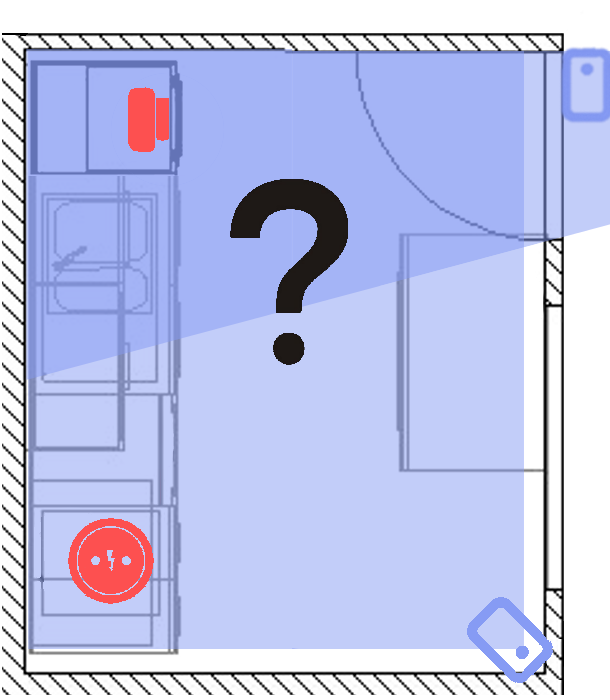
\includegraphics[scale=0.15]{use_case_issue_2.png}
      \end{figure}
    \end{minipage}
  \hfill
  \begin{minipage}{0.65\linewidth}
    %\vspace*{-25.9mm}
    \begin{coloredbox}[black]{Dépendance de présence}
      \footnotesize
      Chaque interaction (sauf présence) doit être recouverte par une interaction de présence.
      \small
      \begin{displaymath}
        \begin{array}{c}
        ~\\
        ~
        \end{array}
      \end{displaymath}
    \end{coloredbox}
    \begin{coloredbox}[black]{Non ubiquité}
      \footnotesize
      Une présence ne peut pas être simultanément détectée dans deux endroits différents.
      \small
      \begin{displaymath}
        \begin{array}{c}
         ~\\ 
         ~
        \end{array}
      \end{displaymath}
    \end{coloredbox}
  \end{minipage}
\end{frame}

\begin{frame}{Rendre explicite le modèle implicite~: Modèle d'infrastructure}
  \addtocounter{framenumber}{-1}
  \begin{minipage}{0.3\linewidth}
      \begin{figure}
        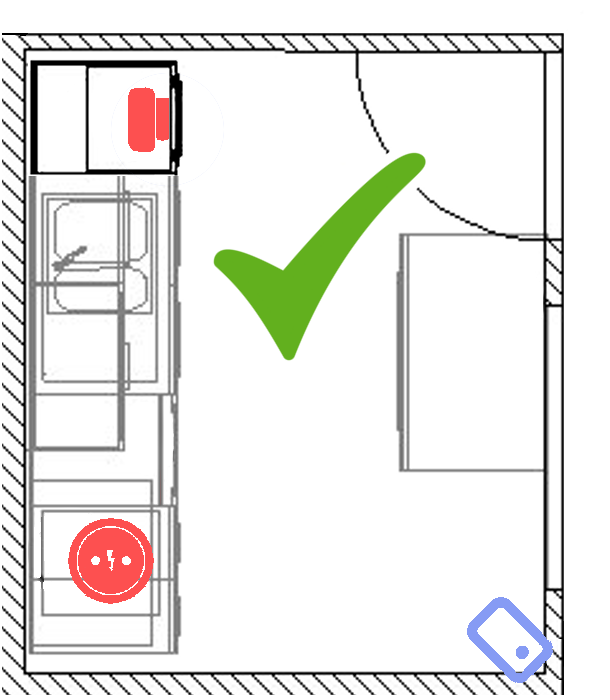
\includegraphics[scale=0.15]{use_case_final.png}
      \end{figure}
    \end{minipage}
  \hfill
  \begin{minipage}{0.65\linewidth}
    \begin{coloredbox}[black]{Dépendance de présence}
      \footnotesize
      Chaque interaction (sauf présence) doit être recouverte par une interaction de présence.
      \small
      \begin{displaymath}
        \begin{array}{c}
          \forall~<k, Kitchen, p>~\in~Log, k \neq Presence~ \Rightarrow \\
          ~~~~\exists~ <Presence, Kitchen, p'>~\in~Log,~p \subseteq p' 
        \end{array}
      \end{displaymath}
    \end{coloredbox}
    \begin{coloredbox}[black]{Non ubiquité}
      \footnotesize
      Une présence ne peut pas être simultanément détectée dans deux endroits différents.
      \small
      \begin{displaymath}
        \begin{array}{c}
          \forall~<Presence, l, p>~\in~Log \Rightarrow \\
          ~~~~\nexists~ <Presence, l', p'>~\in~Log,~l \neq l' \wedge ~p' \cap p \neq \emptyset
        \end{array}
      \end{displaymath}

    \end{coloredbox}
  \end{minipage}
\end{frame}
% **********************************************

% \begin{frame}{Rendre explicite le modèle implicite}
%   % Abstraction de roles de capteurs: {\footnotesize \( e~\in~Event = Kind \times Loc \times Period\)}

%   \begin{minipage}{0.3\linewidth}
%     \onslide<1->{
%       \begin{figure}
%         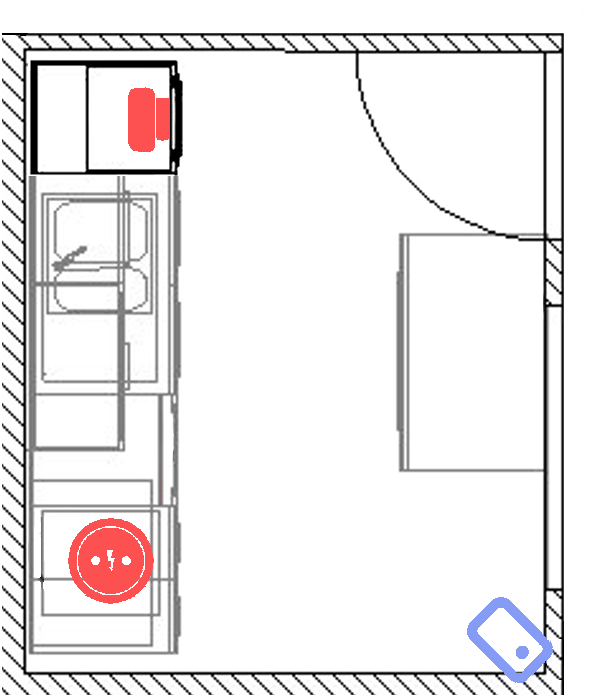
\includegraphics[scale=0.15]{use_case1.png}
%       \end{figure}
%       % \begin{footnotesize}
%       %   \begin{coloredbox}[teal]{Hypothèses}
%       %     \begin{itemize}
%       %     \item Détection de mouvement précède toute autre interaction.
%       %     \item Une présence dans une pièce ne peut pas recouvrir une présence dans une autre pièce.
%       %     \end{itemize}
%       %   \end{footnotesize}
%       }
%     \end{minipage}
%   \hfill
%   \begin{minipage}{0.65\linewidth}
%     \begin{coloredbox}[gray]{Dépendance de présence}
%       \footnotesize
% \onslide<1->{
%       Chaque interaction (sauf présence) doit être recouverte par une interaction de présence.% à la même localisation
%       % Any detected interaction (but presence) must be surrounded by a presence interaction
% }
%       \small
% \onslide<2->{
%       \begin{displaymath}
%         \begin{array}{c}
%           \forall~<k, Kitchen, p>~\in~Log, k \neq Presence~ \Rightarrow \\
%           ~~~~\exists~ <Presence, Kitchen, p'>~\in~Log,~p \subseteq p' 
%         \end{array}
%       \end{displaymath}
% }
%     \end{coloredbox}
%     %\vfill
%     \begin{coloredbox}[gray]{Non ubiquité}
%       \footnotesize
% \onslide<1->{
%       Une présence ne peut pas être simultanément détectée dans deux endroits différents.
% }
%       \small
% \onslide<3->{
%       \begin{displaymath}
%         \begin{array}{c}
%           \forall~<Presence, l, p>~\in~Log \Rightarrow \\
%           ~~~~\nexists~ <Presence, l', p'>~\in~Log,~l \neq l' \wedge ~p' \cap p \neq \emptyset
%         \end{array}
%       \end{displaymath}
% }
%     \end{coloredbox}
%   \end{minipage}
 
% \end{frame}
% **********************************************
% **********************************************
\begin{frame}[fragile]{Validation avec le projet pilote de Domassist}
%\begin{minipage}[t]{0.45\linewidth}
\begin{coloredbox}[black]{Assistance domiciliaire pour personnes âgées}
 % Aims: Aging in place\linebreak
  %\vfill
\footnotesize
  Services définis par des ergothérapeutes, psychologues, experts en vieillissement.\\%\linebreak
  %Activities defined by experts in occupational therapy and psychology and aging\linebreak
  %\vfill
  
  \begin{itemize}
  \item Applications de surveillance des activités du quotidien.
  \item Applications de sécurité du domicile et de l'utilisateur.
  \end{itemize}
  %\vfill
  Étude conduite avec 24 participants vivant seuls pendant 9 mois.
  %Field study: conducted with 24 older participants for a period of 9 months
\end{coloredbox}
\vfill
%\end{minipage}
%\hfill
%\begin{minipage}[t]{0.45\linewidth}
   \begin{table}[!h]
    \begin{scriptsize}
      \begin{tabular}{| c | c |} \hline
        {\bf Name} & {\bf Rule} \\ \hline \hline
        Dépendance de présence & 
$\forall~<i, l, p>~\in~Log, i \neq Presence~ \Rightarrow$\\
        &$~~~\exists~ <Presence, l, p'>~\in~Log,~p \subseteq p'$
%\end{displaymath} 
\\ \hline
        Porte restée ouverte & $\forall~<Opening, l, p>~\in~Log \Rightarrow  \# p < MAX$  \\ \hline
        Non ubiquité & $\forall~<Presence, l, p>~\in~Log \Rightarrow$ \\
     &$~~~~\nexists~ <Presence, l', p'>~\in~Log,~l \neq l' \wedge ~p' \cap p \neq \emptyset$ \\ \hline
         Taux de déclenchement & $\forall~<k, l, p>~\in~Log \Rightarrow$ \\
     &$~~~~~\# (p - Prev(<k, l, p>)) < MAX$ \\ \hline
      \end{tabular}
    \end{scriptsize}
    \vspace{5mm}
    \label{scenario-fig}
    %\caption{Example de scénarios de services d'assistance.}
  \end{table}
%\end{minipage}
\end{frame}
% **********************************************
\begin{frame}{Fiabilité~: Résultats }
  \begin{minipage}[h]{0.45\linewidth}
    \begin{coloredbox}[black]{
        Non-conformités permanentes~:%}
      }
      \onslide<2->{
        %\begin{figure}
          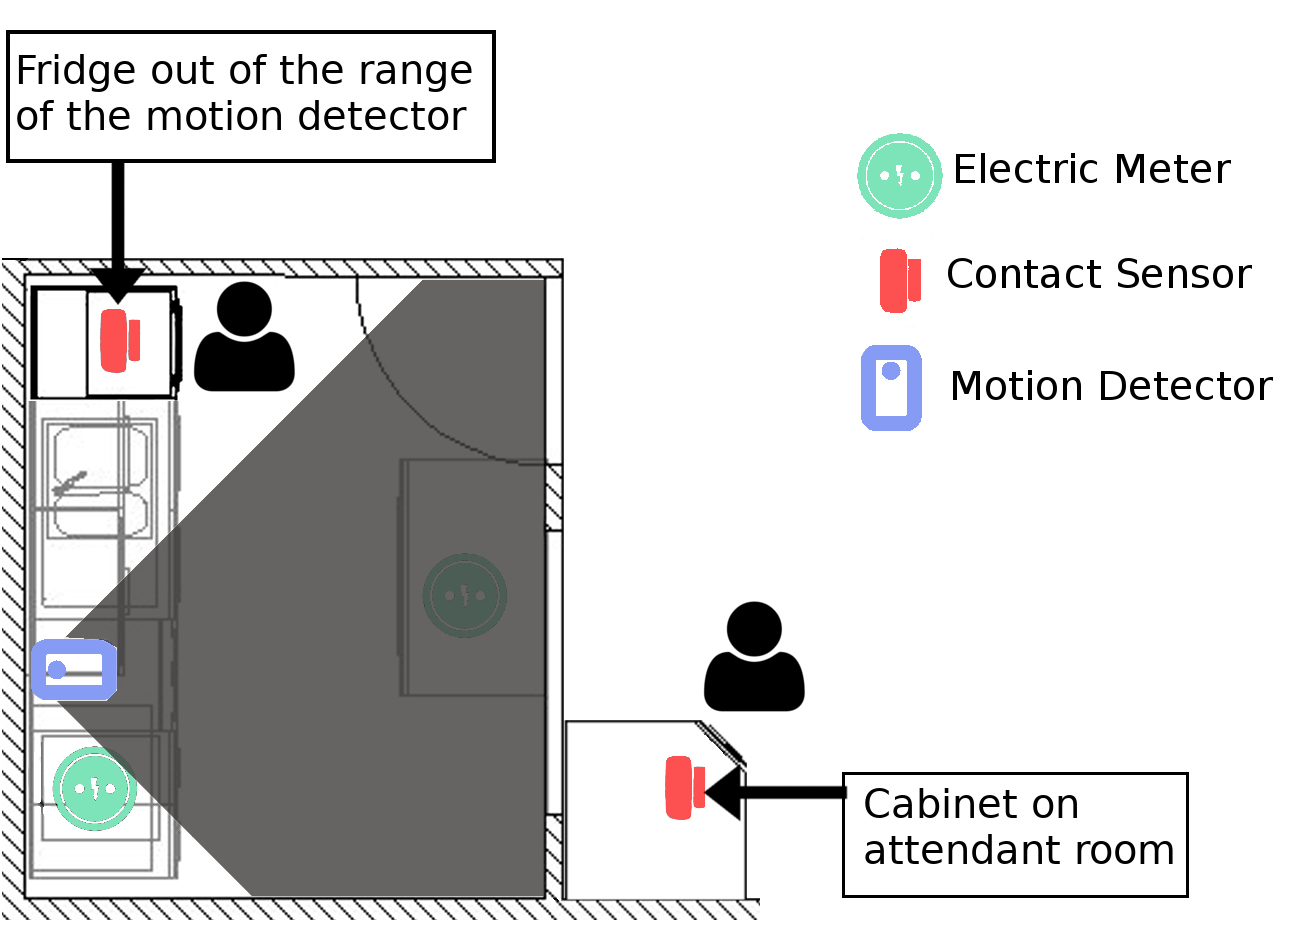
\includegraphics[scale=0.125]{nconf3.png}
          %\label{fig:map}
        %\end{figure}
        \begin{itemize}[label=$\rightarrow$,font=\LARGE \color{black}]
        \item Adapter le modèle.
        \item Repositionner le capteur. 
        \end{itemize}
      }
    \end{coloredbox}
    
  \end{minipage}
  \hfill
  \begin{minipage}[h]{0.45\linewidth}
    \begin{coloredbox}[black]{
        Non-conformités émergentes~: }
      \begin{small}
\onslide<3->{
        \begin{itemize}
        %\item \textbf{Porte restée ouverte~:} \\Chute du capteur de contact.
        \item Chute du capteur de contact.
        %\item \textbf{Dépendance de présence~:}\\Capteur de mouvement défaillant.
        \item Capteur de mouvement défaillant.
%        \item \textbf{Non ubiquité~:}\\Latence des detecteurs de mouvements.

        \end{itemize}
        \vfill
        \begin{itemize}[label=$\rightarrow$,font=\LARGE \color{black}]
        \item Intervention d'un technicien.
        \end{itemize}
}
      \end{small}
    \end{coloredbox}
  \end{minipage}
\end{frame}
% **********************************************
\begin{frame}{Synthèse~: Assurer la fiabilité du contexte\\
Modèle d'infrastructure explicite sous forme de règles~\cite{carteron2016improving}
}
\begin{coloredbox}[checked]{Conformité d'une installation avec un modèle}
%Conformité d'une installation avec un modèle:
  \begin{itemize}%[<+->]
  \item Certifie l'installation.
  \item Guide l'installation.
  \item Application certifiée pour un modèle/installation.
  \end{itemize}
\end{coloredbox}
\vfill
\begin{coloredbox}[checked]{Vérification continue}
%Vérification continue:  
  \begin{itemize}
  \item Détection des pannes.
  \item Aide au diagnostic.
  \end{itemize}
\end{coloredbox}
\vfill

%~\cite{carteron2016improving}
\end{frame}
% **********************************************

% **********************************************